\documentclass[../main.tex]{subfiles}

\begin{document}

\chapter{Demonstration of the query interface that has been built}
\label{chapter:demonstration}

The query program is called ``Solarman'', and there exists two web based interfaces that can be used to interact with it.

\section{Natural Language Interface}

The English Natural Language query interface can be accessed via this URL:

\url{http://speechweb2.cs.uwindsor.ca/solarman2/demo_sparql.html}

%Screenshot of the page

\begin{figure}[h]
\centering
\frame{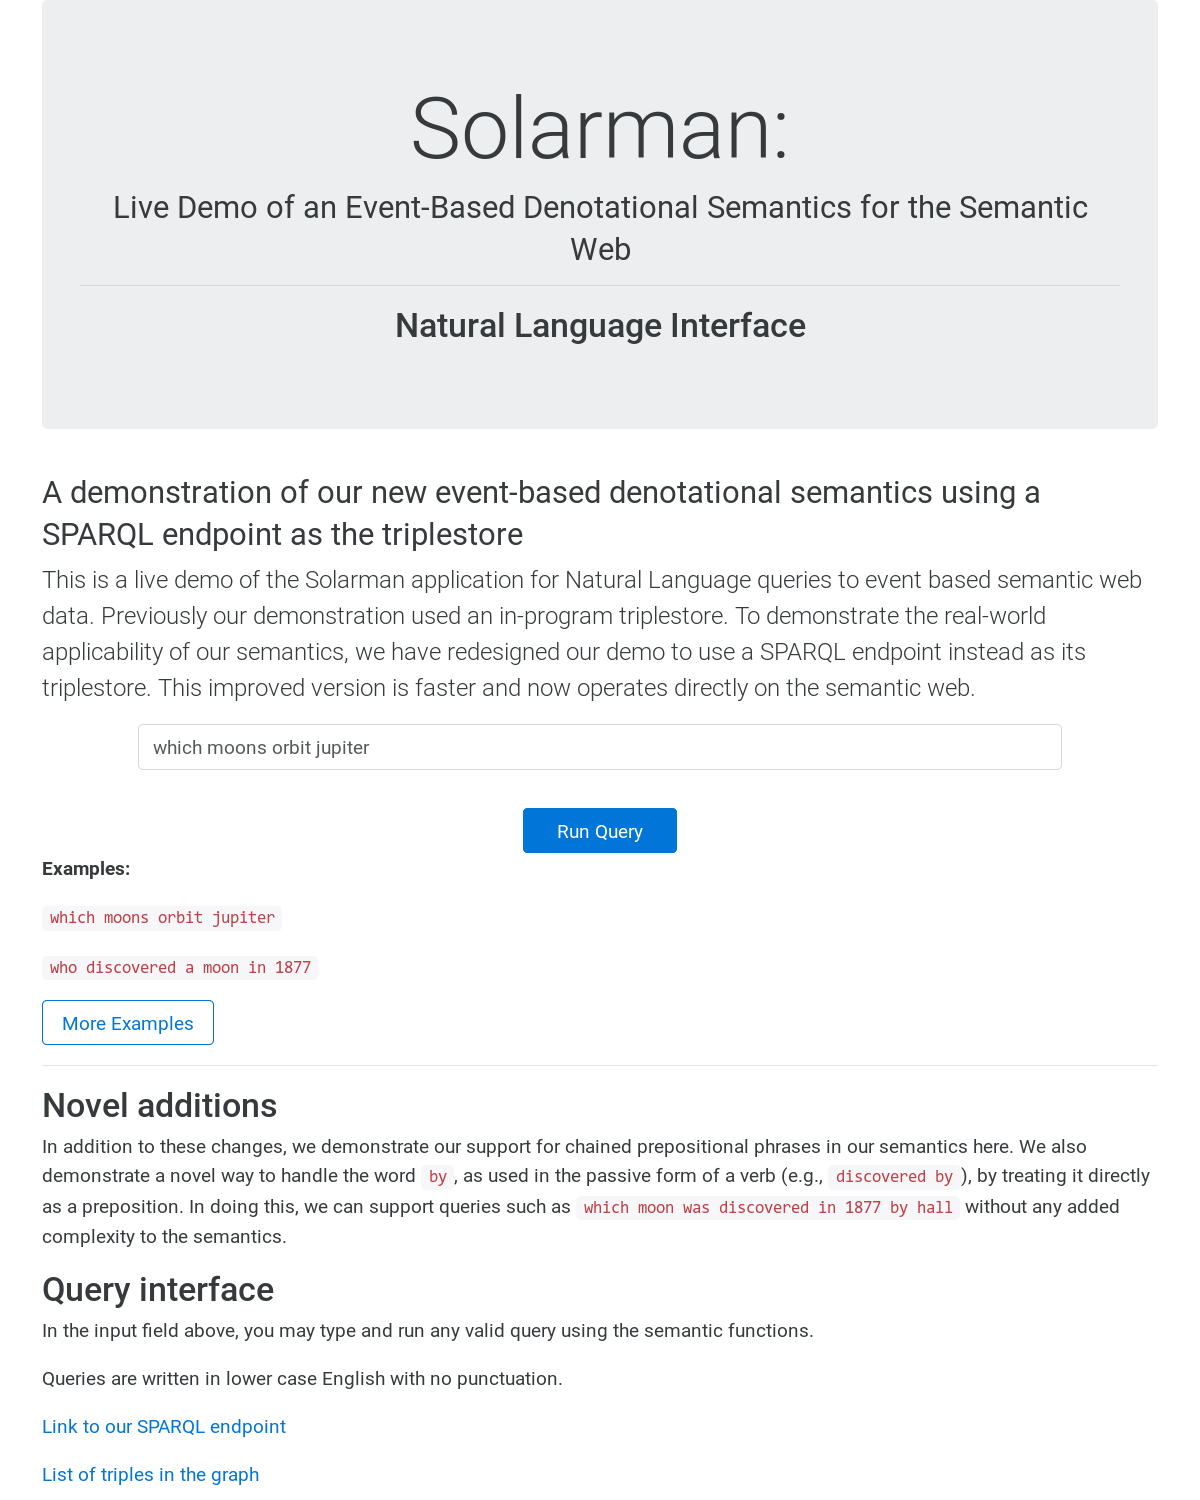
\includegraphics[width=\textwidth]{natlang4}}
\caption{Screenshot of English Natural Language Interface}
\end{figure}
In the text box labeled ``Enter query here'', English queries about the Solar system can be entered to be evaluated.  This is accomplished using the {\em Common Gateway Interface}, or {\em CGI}, to directly execute the ``Solarman'' program on the server with the given query as an argument.  Internally, Solarman is configured to use a Virtuoso\cite{virtuoso} RDF database as its SPARQL endpoint.

Traversing the ``More Examples'' link will bring up a page that contains a full list of the words that can be used in queries, along with a list of example queries that can be used.

Some example queries that use prepositional phrases include:

\begin{itemize}
	\item \texttt{what moon was discovered by one person in 1877}
	\item \texttt{what planet is orbited by a moon that was discovered in 1684}
	\item \texttt{what was discovered in 1877 in us\_naval\_observatory with a \\ telescope}
	\item \texttt{how many moons were discovered in 1938}
	\item \texttt{where were the moons that were discovered by hall or kuiper in \\ 1877 discovered}
	\item \texttt{which moons that orbit a planet that orbits a sun were discovered \\ by one person at a place with a telescope}
	\item \texttt{how were the moons that were discovered with two telescopes\\ discovered}
\end{itemize}

%%

\section{Direct Query Interface}

In addition, a ``Direct Query Interface'' is provided that allows users to directly interact with the parser combinators and semantic functions by chaining them together to form queries.  This is useful tool to explore and understand the semantics.  It can be accessed via this URL:

\url{http://speechweb2.cs.uwindsor.ca/solarman2/demo_sparql_direct.html}

\begin{figure}[h]
	\centering
	\frame{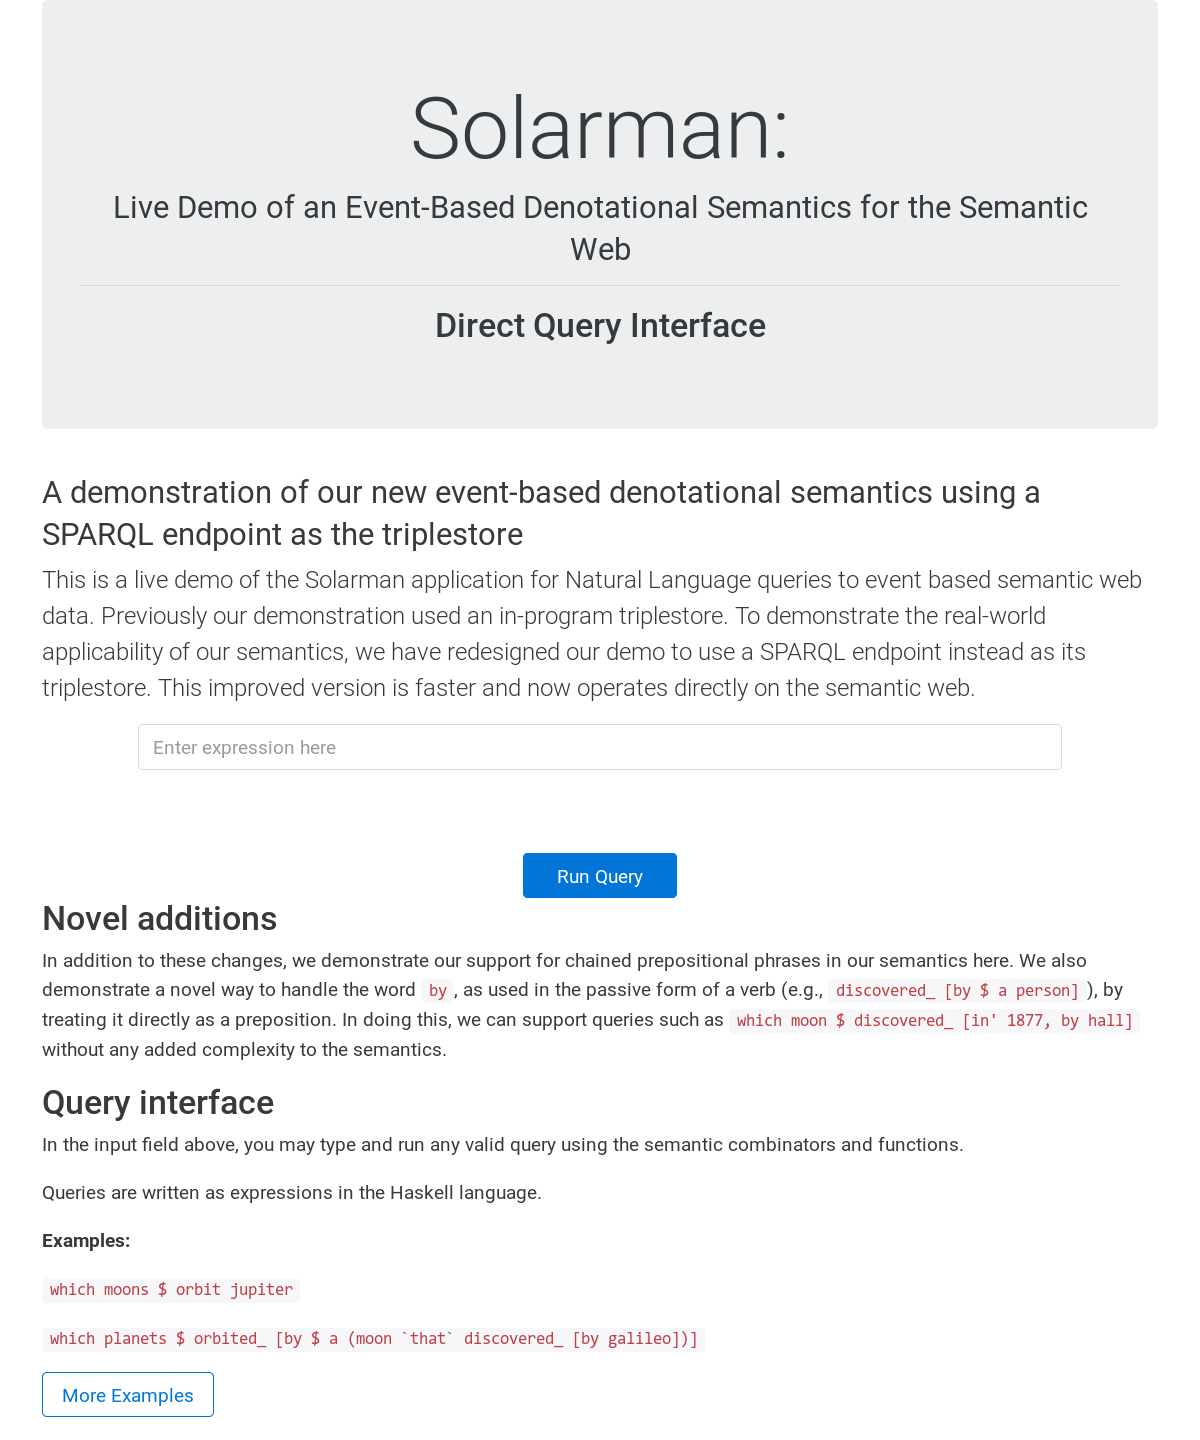
\includegraphics[width=\textwidth]{directquery3}}
	\caption{Screenshot of Direct Query Interface}
\end{figure}

The Direct Query Interface is implemented using Safe Haskell\cite{safehaskell}, an extension of the Haskell language that restricts the functions that can be evaluated
to a safe subset that is suitable for executing untrusted code.  This makes the Direct Query Interface suitable for use on public-facing websites, preventing external users from executing malicious code using the interface.  For example, the expression \texttt{System.IO.readFile "/etc/passwd"} is disallowed under this scheme as both the Haskell \texttt{Prelude} and \texttt{System.IO} modules are by default not trusted.

Examples of queries that can be performed with the Direct Query Interface:
\begin{itemize}
	\item \texttt{when' \$ something \$ discovered\_ [at mt\_wilson]} \\(English: ``when was something discovered at mt\_wilson'')
	\item \texttt{how' \$ discovered \$
	\subitem the (thing `that` discovered\_ [at flagstaff])} \\(English: ``how was the thing that was discovered at flagstaff discovered'')
	\item \texttt{what \$ discovered\_ [in' 1877, at us\_naval\_observatory]} \\(English: ``what was discovered in 1877 at us\_naval\_observatory'')
	\item \texttt{which planet \$ orbited\_ 
		\subitem [by \$ a (moon `that` discovered\_ [in' 1684])]} \\(English: ``what planet is orbited by a moon that was discovered in 1684'')
	\item \texttt{which
		\subitem (liftM2 intersect\_fdbr vacuumous  (moon `that` orbits jupiter))
		\subitem \$ discovered\_ [by \$ nicholson `termor` hall, \subsubitem with \$ a telescope, in' 1938, \subsubitem at \$ mt\_wilson `termor` mt\_hopkins]}\\(English: ``which vacuumous moon that orbits jupiter was discovered by nicholson or hall with a telescope in 1938 in mt\_wilson or mt\_hopkins'')
\end{itemize}

\subsection{Verb voices}

When using transitive verbs in the Direct Query Interface, the appropriate voice of the verb must be selected.  Both the ``discover'' and ``orbit''
transitive verbs are supported.  The available voices are summarized as follows:

\begin{itemize}
	\item discover is the active voice (e.g. "hall discovered a moon")
	\item discover' is the active voice with support for prepositional phrases, and
	\item discover\_ is the passive voice with prepositional phrases
\end{itemize}

The above voices apply to the ``orbit'' verb as well.

\subsection{Evaluating types}

In addition to evaluating queries, the types of the combinators themselves and their results may also be evaluated by prepending the query with
``\texttt{:t}''.  For example:

\begin{itemize}
	\item ``\texttt{:t moon}'' returns ``\texttt{moon :: IO FDBR}''
	\item ``\texttt{:t a moon}'' \subitem returns ``\texttt{a moon :: IO [(String,  t2)] $\rightarrow$ IO [(String,  t2)]}''
	\item ``\texttt{:t by}'' returns ``\texttt{by :: t $\rightarrow$ ([[Char]],  t)}''
	\item ``\texttt{:t discovered'}'' \subitem returns ``\texttt{discovered' :: (IO FDBR $\rightarrow$ IO FDBR) $\rightarrow$ \subsubitem [([[Char]],  IO FDBR $\rightarrow$ IO FDBR)] $\rightarrow$ IO FDBR}''
	\item ``\texttt{:t vacuumous}'' returns ``\texttt{vacuumous :: IO FDBR}''
\end{itemize}

In the above query results, \texttt{FDBR} refers to the ``Function Defined By Relation'' construct which is explained in Chapter \ref{chapter:semantics}.  A value of type
\texttt{IO FDBR} represents an ``IO Action'', when executed, yields a value of type \texttt{FDBR}.  In our semantics, the \texttt{FDBR} type is defined as \texttt{[(String, [String])]}.
The type $\mathtt{a \rightarrow b}$ is used to denote a function from type $\mathtt{a}$ to type $\mathtt{b}$.

The Haskell language deduces the most general type declaration possible for a given function definition.  If certain components of an input value aren't used,
those components will be replaced with a {\em type variable} when possible.  This can be seen above in the queries for \texttt{:t a moon} and \texttt{:t by}.
Neither of these expressions use the list of events associated with the input FDBR, and therefore the type declaration was generalized,
substituting a type variable for the list of events.  The type variable is allowed to be bound to any type, subject to type constraints.
For example, in ``\texttt{:t a moon}'', if we let \texttt{t2 = [String]}, then \texttt{a moon :: IO [(String, [String])]} and hence \texttt {a moon :: IO FDBR}.

\subsection{Result formatting}

The results of the Direct Query Interface are formatted for easier viewing.  In particular, in each ``FDBR'', each result pair is on its own line, making
it clear which entities are connected with which events.

\section{XSaiga Package}

``Solarman'' is also included as part of the XSaiga package that we have uploaded to {\em Hackage}, an online repository of Haskell libraries and software\cite{XSaiga:2016}.
It is available at this URL:

\url{https://hackage.haskell.org/package/XSaiga}

To install the XSaiga package, the GHC compiler version 8.0.1 or higher is required.  With the {\em cabal} command, execute the following at a terminal:

\begin{code}
	> cabal update
	> cabal install XSaiga
\end{code}

The XSaiga code resides inside the XSaiga namespace, and includes the parser, Solarman and its semantics, and a local triplestore in the module ``LocalData'' containing
all of the RDF triples in a list.  

\section{Accessibility}

Both interfaces are also designed to be accessible, supporting programs such as screen readers in order to accommodate those with disabilities.
This was accomplished using the {\em WAVE Web Accessibility Evaluation Tool}\cite{wave} and {\em AChecker IDI Web Accessibility Checker}\cite{achecker} to validate the interfaces for accessibility.

\section{SPARQL Endpoint}
The SPARQL endpoint that Solarman uses can be accessed via this URL:

\url{http://speechweb2.cs.uwindsor.ca/sparql}

We use the Virtuoso RDF triplestore and its SPARQL interface\cite{virtuoso} in our demonstration.  To replicate our setup,
first install the Virtuoso software for your operating system.  Next, obtain a database dump of our triplestore
in ``n-Triples'' format\cite{w3cntriples} using this URL:

\url{http://speechweb2.cs.uwindsor.ca/solarman2/triples.nt}

Finally, use the ``bulk import'' mechanism in Virtuoso Conductor to import our triples into your triplestore, selecting the \texttt{triples.nt} file.
Our semantics can use any SPARQL interface, so the Virtuoso triplestore may be substituted with any number of alternatives, including Apache Jena\cite{jena2013apache}. 

\end{document}